\chapter[Comparativo]{Custo e Comparação}

\section{Custo da GreenHome}

Os recursos solicitados para o presente projeto visam principalmente atender as exigências dos futuros compradores e manter os quatros pilares de uma casa sustentável, que são eles: segurança, economia energética, conforto e sustentabilidade. O custo total\footnote{O custo total irá variar de acordo com a cotação das moedas e com a escolha do terreno} da GreenHome ficou em, aproximadamente, um milhão trezentos e doze mil cento e vinte três reais (R\$1.312.123,06).

\begin{table}[H]
\centering
\begin{tabular}{|c|c|}
\hline 
\textbf{Área} & \textbf{Custo}\tabularnewline
\hline 
\hline 
Automação & R\$ 60.000,00\tabularnewline
\hline 
Energia & R\$ 116.000,00\tabularnewline
\hline 
Software & R\$ 2.000,00\tabularnewline
\hline 
Estrutura & R\$ 909.897,06\tabularnewline
\hline 
Terreno & R\$ 221.226,00\tabularnewline
\hline 
\textbf{Total} & R\$ 1.312.123,06\tabularnewline
\hline 
\end{tabular}
\caption{Custo em relação as áreas de pesquisa da GreenHome.}
\end{table}


\section{Comparativo entre os Concorrentes}

Abaixo há uma descrição das casas que são as possíveis concorrentes da GreenHome. Logo após a descrição de cada casa, há um quadro comparativo entre as casas.

\subsection{Casa Aqua}

A Casa Aqua é um projeto apresentado pela empresa Leroy Merlin, possui 40 \si{\meter}$^2$ e tem um custo por volta de R\$ 45.000,00 que tem por prioridade mostrar aos clientes da loja como montar uma casa mais econômica e ecológica utilizando materiais que prejudicam menos o meio ambiente, além de apresentar propostas de redução no consumo de água e energia.

\begin{figure}[H]
\begin{center}
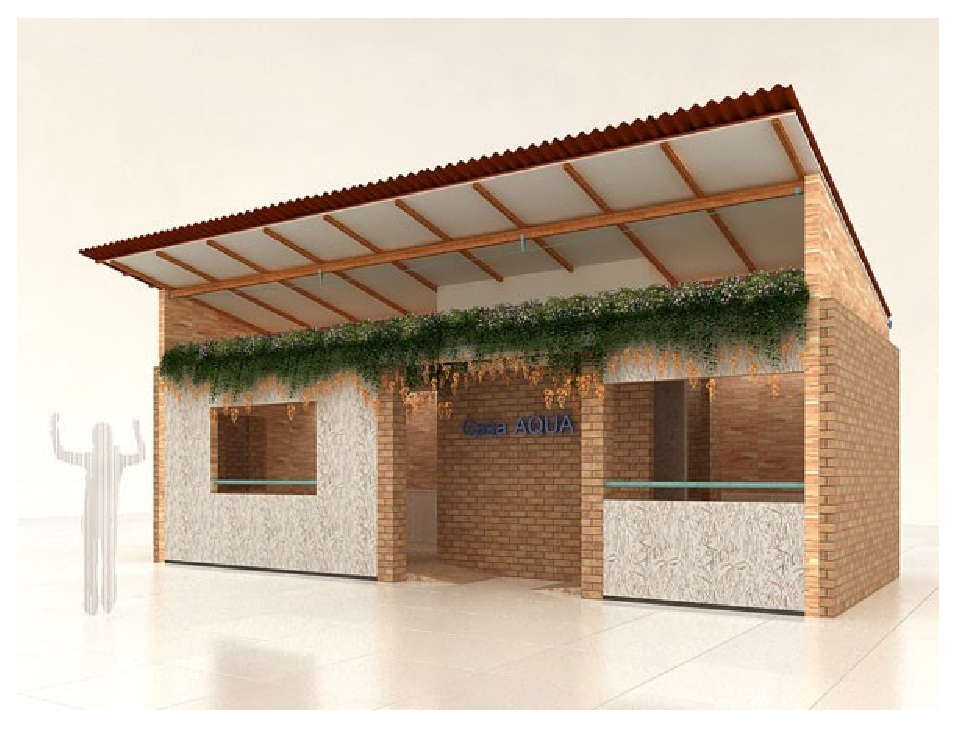
\includegraphics[keepaspectratio,scale=0.6]{figuras/modelocasaaqua.jpg.eps}
\caption{Modelo Casa Aqua.}
\end{center}
\end{figure}

\subsection{Unidade habitacional com selo azul}

	Essa unidade faz parte de um estudo da universidade do amazonas, com residências de 200\si{\meter}$^2$ que mostra dentre vários critérios opcionais e obrigatórios a serem implantados na residência de acordo com a vontade do  contratante para atingir um selo de  importância sustentável. Dentre os itens de caráter obrigatório encontram se preocupação com infraestrutura, impactos, paisagismo, local para coleta seletiva do lixo, equipamentos de lazer, com orientação ao sol e ventos, entre outros.

\subsection{Casa de Campinas com selo leed for homes}

	Essa casa de campinas de 450\si{\meter}$^2$ foi planejada para comportar diversas soluções sustentáveis, desde a utilização de painéis solares, meios para reutilização da água cinza além de uma extrema preocupação com o material utilizado em sua construção, chegando a aplicar por exemplo apenas a  utilização de madeira reflorestada, isso  permitiu que esta fosse a primeira casa na América Latina a receber o selo leed for homes.

\begin{figure}[H]
\begin{center}
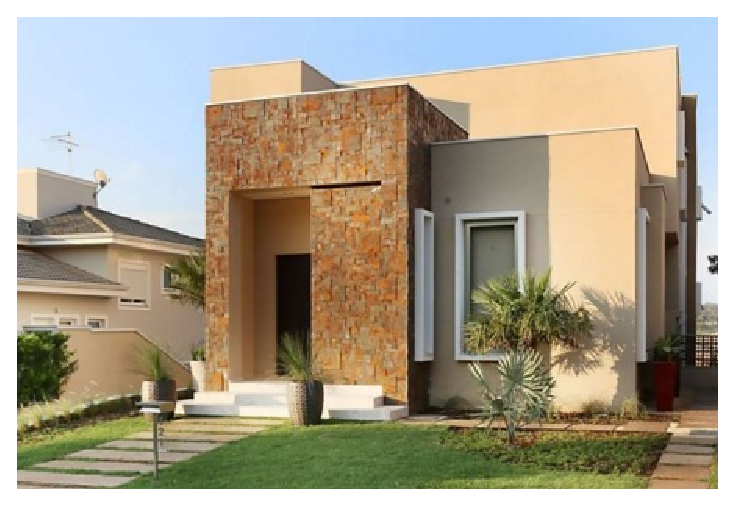
\includegraphics[keepaspectratio,scale=0.6]{figuras/modelocasacampinas.eps}
\caption{Modelo Casa de Campinas com selo leed for homes.}
\end{center}
\end{figure}


\subsection{Casa no Jardim Botânico}

Esse casa no jardim botânico de 1000\si{\meter}$^2$ se encontra em uma área regularizada e apresenta os padrões de uma casa normal, ou seja, sem implementação de recursos/itens que buscam uma sustentabilidade para a residência.

\begin{figure}[H]
\begin{center}
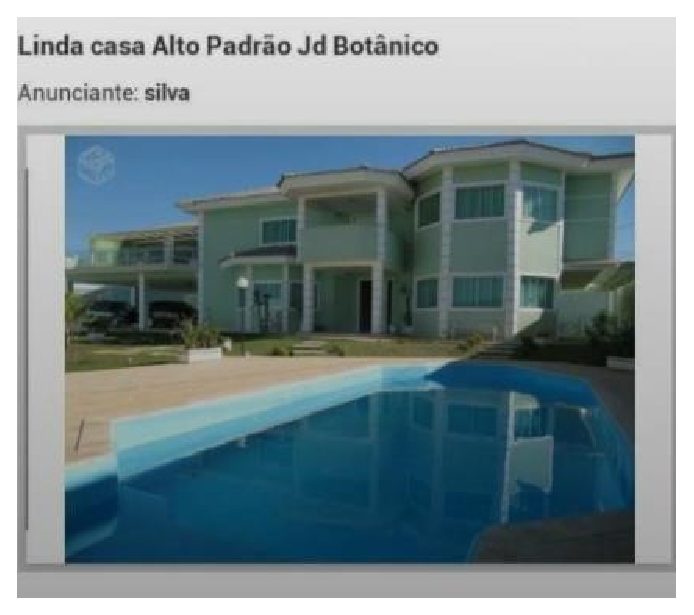
\includegraphics[keepaspectratio,scale=0.6]{figuras/casajardimbotanico.eps}
\caption{Modelo Casa no Jardim Botânico.}
\end{center}
\end{figure}


\subsection{Tabela comparativa}	

	A tabela a seguir mostra a GreenHome sendo comparada com Casas Sustentáveis, e também com uma casa comum no condomínio Jardim Botânico. 

\begin{table}[H]
\centering
% Preview source code for paragraph 0

\begin{sideways}
\begin{tabular}{|c|c|c|c|c|c|}
\cline{2-6} 
\multicolumn{1}{c|}{} & \multirow{3}{*}{Casa Aqua} & Unidade habitacional & Casa de Campinas & Casa no  & \multirow{3}{*}{Green home}\tabularnewline
\multicolumn{1}{c|}{} &  & com selo & com selo & \multirow{2}{*}{Jardim Botânico} & \tabularnewline
\multicolumn{1}{c|}{} &  & casa azul & leed for homes &  & \tabularnewline
\hline 
Materiais Sustentáveis & Sim & Sim & Sim & Não & Sim\tabularnewline
\hline 
Reutilização da & \multirow{2}{*}{} & \multirow{2}{*}{Sim} & \multirow{2}{*}{Sim} & \multirow{2}{*}{Não} & \multirow{2}{*}{Sim}\tabularnewline
 água cinza &  &  &  &  & \tabularnewline
\hline 
Utilização da  & \multirow{2}{*}{Sim} & \multirow{2}{*}{Sim} & \multirow{2}{*}{Sim} & \multirow{2}{*}{Não} & \multirow{2}{*}{Sim}\tabularnewline
água da chuva &  &  &  &  & \tabularnewline
\hline 
Implantação de  & \multirow{2}{*}{Sim} & \multirow{2}{*}{Sim} & \multirow{2}{*}{Sim} & \multirow{2}{*}{Não} & \multirow{2}{*}{Sim}\tabularnewline
placas solares &  &  &  &  & \tabularnewline
\hline 
Implementação de & \multirow{2}{*}{Não} & \multirow{2}{*}{Não} & \multirow{2}{*}{Não} & \multirow{2}{*}{Não} & \multirow{2}{*}{Sim}\tabularnewline
 energia eólica &  &  &  &  & \tabularnewline
\hline 
Utilização de  & \multirow{2}{*}{Não} & \multirow{2}{*}{Não} & \multirow{2}{*}{Não} & \multirow{2}{*}{Não} & \multirow{2}{*}{Sim}\tabularnewline
Composteira &  &  &  &  & \tabularnewline
\hline 
Automação & Não & Sim & Sim & Não & Sim\tabularnewline
\hline 
Sistema de segurança & Não & Sim & Sim & Não & Sim\tabularnewline
\hline 
Preço/m2 & R\$ 1.125,00/m2 & R\$ 650,00/m2 & R\$ 2.222,22/m2 & R\$ 1.400,00/m2 & R\$ 5467,00/m2\tabularnewline
\hline 
\end{tabular}
\end{sideways}
\caption{Comparativo entre a GreenHome e outras casas.}
\end{table}